Natural Language Processing (NLP) is a sub-field of Artificial Intelligence (AI) that deals with the understanding and generation of natural human languages. Natural language

Recently many of the tasks traditionally addressed by statistical NLP methods are moving towards the adoption of neural networks to parameterize more expressive models of language. This includes tasks like machine translation, dialogue modelling, abstract summarisation, document classification etc.

The problem this thesis attempts to tackle is the neural disentanglement of style and content in text. We evaluate the efficacy of our method by generating text conditioned on any of a given set of discrete labels (used interchangeably with attribute or style henceforth). This is analogous to style transfer in computer vision \citep{gatys2016image}. The requirement of the style transfer task in the vision domain is to transfer the visual style from one image to the other, as illustrated in Figure \ref{fig:style-transfer-vision}. Stylistic transfer in text is based on a similar premise, wherein, given an arbitrary body of text and a predefined style governed by a set of one or more attributes like sentiment, emotion, tense, authorship etc., a new body of text can be generated such that it incorporates all of the predefined attributes its generation is being conditioned on.

\begin{figure}[ht]
	\centering
	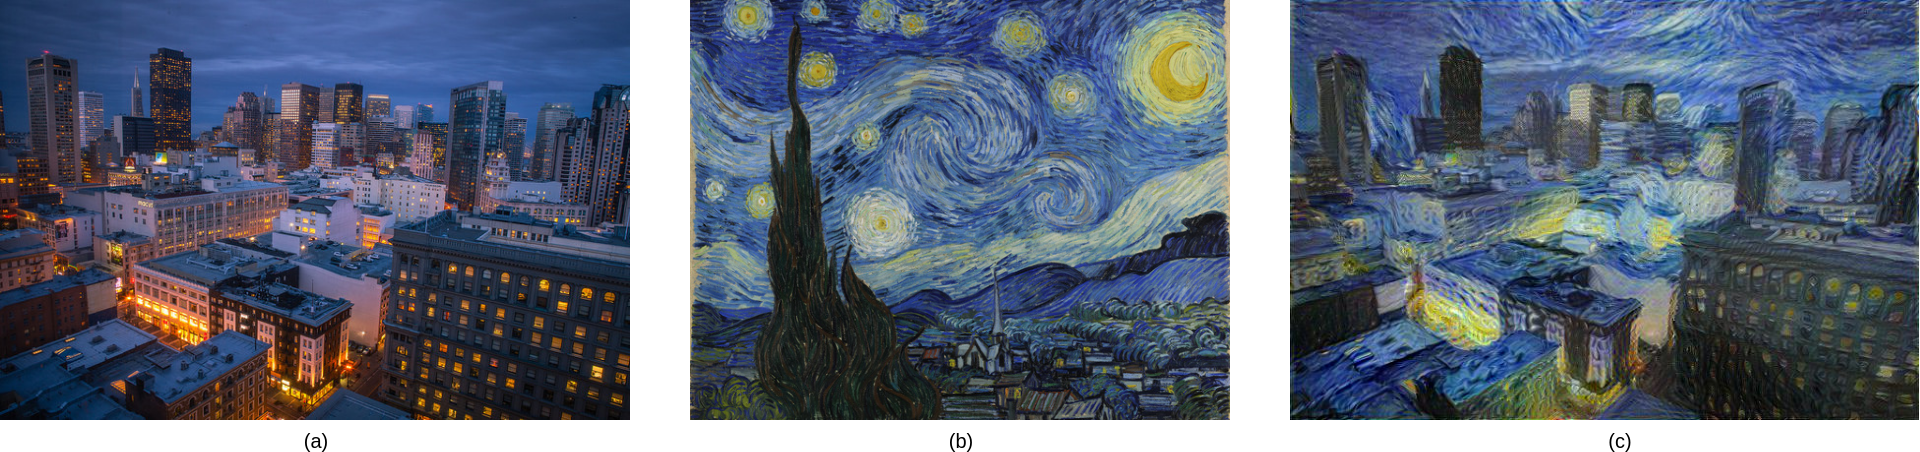
\includegraphics[width=\textwidth]{images/style-transfer-vision.png}
	\imgsrc{\url{https://github.com/fzliu/style-transfer}}
	\caption{\label{fig:style-transfer-vision}Sample of vision style transfer. Image (a) provides the content, image (b) provides the style and image (c) is the final generated image}
\end{figure}


\begin{table}[ht]
	\centering
	\begin{tabular}{ | p{.45\linewidth} | p{.45\linewidth} | }
		\hline
		\textbf{Input}                                              & \textbf{Output}                                      \\
		\hline \hline
		i will bite thee by the ear for that jest .                 & i ’ ll bite you by the ear for that joke .           \\
		\hline
		what further woe conspires against mine age ?               & what ’ s true despair conspires against my old age ? \\
		\hline
		how doth my lady ?                                          & how is my lady ?                                     \\
		\hline
		hast thou slain tybalt ?                                    & have you killed tybalt ?                             \\
		\hline
		an i might live to see thee married once , i have my wish . & if i could live to see you married, i ’ ve my wish . \\
		\hline
		benvolio , who began this bloody fray ?                     & benvolio , who started this bloody fight itself ?    \\
		\hline
		what is your will ?                                         & what do you want ?                                   \\
		\hline
		call her forth to me .                                      & bring her out to me .                                \\
		\hline
	\end{tabular}
	\imgsrc{\cite{xu2012paraphrasing}}
	\caption{Authorship style transfer from Shakespearean plays to modern english}
	\label{tab:paraphrasing-for-style-results}
\end{table}

The task of style transfer in context of text was first introduced by \cite{xu2012paraphrasing} as a statistical model that attempted to paraphrase bodies of text in a different style using a simple phrase replacement strategy. An few examples from this paper are shown in Table \ref{tab:paraphrasing-for-style-results}. Although fairly crude, this retrieve and replacement strategy is effective, given a large dataset with enough phrase context overlap. Since the overwhelming adoption of neural network based models in the NLP community, there have been several new bodies of work that break new ground in this area. These are discussed in the chapter dedicated to related works.


\section{Problem Statement}

The objective of this thesis is to perform an exploratory analysis of previous methods and test novel hypotheses that tackle the problem of the disentanglement of latent spaces of artificial neural networks and its applications to linguistic style transfer.

We operate under the following constraints and assumptions in our formulation of the problem:

\begin{itemize}
	\item The model is singular, with no conditional execution branch based on desired attribute. i.e. there is only one decoder and the number of decoders does not scale with the number of distinct transferable attributes.
	\item The corpus of styles are non-parallel i.e. for instance, there are no pre-defined pairs of $(document_1, document_2)$ for style labels $\in (1, 2)$, as would be commonly seen in neural machine translation corpora.
	\item The corpora is annotated with the current attribute each document possesses e.g. each document has a corresponding `positive'/`negative' label if the task is to perform sentiment transfer.
	\item Optionally, a lexicon of words that are statistically likely to be associated with each distinct class label would be useful, primarily to evaluate how well content has been preserved in a generated sentence without penalizing a potential change in vocabulary caused by the transferring of style.
\end{itemize}


\section{Contributions}

Our main contributions in this work can be stated as follows:

\begin{itemize}
	\item We present a comprehensive review of the current literature in linguistic style transfer. It is a quickly evolving sub-area in NLP and a significant amount of work has been done in the last two years.
	\item We propose a combination of methods that have worked well independently, including using adversarial learning and multi-task learning objectives as regularisations on the latent space of neural models.
	\item We propose the usage of a novel bag-of-words adversary and a style dropout regularization that are aimed at further increasing the potency of latent space disentanglement and auto-encoding accuracy. Our model is novel in the aspect of a dual-adversary regularisation as well.
	\item We empirically show that embeddings in the latent space are regularized like we intend them to be, a feature that is absent in contemporary approaches that use discrete labels or embedding matrices to represent style.
	\item We devise new metrics to evaluate text content preservation quantitatively, which is still an open research problem, since the corpora used is non-parallel. Most of the contemporary work either do not measure text content preservation or use human evaluation, which is time consuming.
	\item We implement our model and empirically show that our model outperforms current state-of-the-art models in neural text attribute style transfer, despite not explicitly training with a style transfer objective.
	\item Our model is open-source for inspection, improvements, extensions and replicability.
\end{itemize}

The next chapter will delve deeper into the background required for an understanding of the models we implement and evaluate.
